% Options for packages loaded elsewhere
\PassOptionsToPackage{unicode}{hyperref}
\PassOptionsToPackage{hyphens}{url}
%
\documentclass[
]{article}
\usepackage{lmodern}
\usepackage{amssymb,amsmath}
\usepackage{ifxetex,ifluatex}
\ifnum 0\ifxetex 1\fi\ifluatex 1\fi=0 % if pdftex
  \usepackage[T1]{fontenc}
  \usepackage[utf8]{inputenc}
  \usepackage{textcomp} % provide euro and other symbols
\else % if luatex or xetex
  \usepackage{unicode-math}
  \defaultfontfeatures{Scale=MatchLowercase}
  \defaultfontfeatures[\rmfamily]{Ligatures=TeX,Scale=1}
\fi
% Use upquote if available, for straight quotes in verbatim environments
\IfFileExists{upquote.sty}{\usepackage{upquote}}{}
\IfFileExists{microtype.sty}{% use microtype if available
  \usepackage[]{microtype}
  \UseMicrotypeSet[protrusion]{basicmath} % disable protrusion for tt fonts
}{}
\makeatletter
\@ifundefined{KOMAClassName}{% if non-KOMA class
  \IfFileExists{parskip.sty}{%
    \usepackage{parskip}
  }{% else
    \setlength{\parindent}{0pt}
    \setlength{\parskip}{6pt plus 2pt minus 1pt}}
}{% if KOMA class
  \KOMAoptions{parskip=half}}
\makeatother
\usepackage{xcolor}
\IfFileExists{xurl.sty}{\usepackage{xurl}}{} % add URL line breaks if available
\IfFileExists{bookmark.sty}{\usepackage{bookmark}}{\usepackage{hyperref}}
\hypersetup{
  pdftitle={Aula 10},
  pdfauthor={Manoel Galdino},
  hidelinks,
  pdfcreator={LaTeX via pandoc}}
\urlstyle{same} % disable monospaced font for URLs
\usepackage[margin=1in]{geometry}
\usepackage{graphicx,grffile}
\makeatletter
\def\maxwidth{\ifdim\Gin@nat@width>\linewidth\linewidth\else\Gin@nat@width\fi}
\def\maxheight{\ifdim\Gin@nat@height>\textheight\textheight\else\Gin@nat@height\fi}
\makeatother
% Scale images if necessary, so that they will not overflow the page
% margins by default, and it is still possible to overwrite the defaults
% using explicit options in \includegraphics[width, height, ...]{}
\setkeys{Gin}{width=\maxwidth,height=\maxheight,keepaspectratio}
% Set default figure placement to htbp
\makeatletter
\def\fps@figure{htbp}
\makeatother
\setlength{\emergencystretch}{3em} % prevent overfull lines
\providecommand{\tightlist}{%
  \setlength{\itemsep}{0pt}\setlength{\parskip}{0pt}}
\setcounter{secnumdepth}{-\maxdimen} % remove section numbering

\title{Aula 10}
\author{Manoel Galdino}
\date{13 de junho de 2023}

\begin{document}
\maketitle

\hypertarget{jogos-repetidosmultiperuxedodos}{%
\section{Jogos
repetidos/multiperíodos}\label{jogos-repetidosmultiperuxedodos}}

\hypertarget{barganha-em-legislaturas}{%
\section{Barganha em Legislaturas}\label{barganha-em-legislaturas}}

O modelo clássico é o de Baron-Ferejohn (1989). O artigo do BF foi tão
profícuo (quase 3 mil citações no Google Scholar) que se tornou a base
para uma série de artigos subsequentes analisando formação e dissolução
de governo, (), bicameralismo (), revisãojudicial (), poder de veto do
executivo (), lobby (), estrutura de classe (), comércio internacional
() entre outros. É portanto fundamental conehcer esse trabalho para
entender os modelos formais feitos em todas essas áreas, além da própria
negociação em legislaturas, tema do artigo.

Mas para entender o trabalho de BF, precisamos saber que adaptam o
modelo de barganha do Rubinstein para \(n\) jogadores e regra da
maioria. O artigo do Rubinstein é mais clássico ainda, pois gerou mais
desenvolvimentos ainda, tendo mais de 7 mil citações no Google Scholar.
Então, antes de entrar na aplicação clássica em CP, vamos primeiro para
o modelo do Rubinstein (1982).

Uma negociação bilateral (entre dois agentes) para dividir um objeto
fixo foi um problema para a teoria dos jogos desde seu início. Embora
seja uma aplicação óbia da teoria dos jogos (como negociar
racionalmente), não havia uma boa solução para esse problema. Foi apenas
com o trabalho de Rubinstein que definitivamente a teoria dos jogos
não-cooperativa achou um caminho para abordar a questão. A solução foi
desenhar um protocolo para as negociações. Na versão do Rubinstein, o
protocolo é que as jogadoras fazem ofertas alternadas de divisão de uma
torta (pie), isto é, quanto irá para cada uma. A torta tem valor 1.
Outra forma de interpretar o jogo é que é um jogo do ultimatum repetido.

Given any x 2 (0; 1), the strategy proÖle fa1 = x; a2 = (accept iff a1
\textless= x) is a Nash equilibrium. So, there are inÖnitely many Nash
equilibria.

ut once player 1 has made an o§er, the optimal strategy for 2 is to
accept any offer a1 \textless{} 1 and he is indifferent with accepting
offer a1 = 1: What can you say about subgame perfect equilibria?

O jogo de uma rodada é o jogo do ultimato. Nesse caso, o equilíbrio de
Nash é \(s_1 = ((1, 0), aceita)\).

No caso de um jogo de duas rodadas, a jogadora 1 poderia oferecer
\((x, 1 - x)\) na primeira rodada. Se 2 aceita, o jogo acaba e essa é a
divisão do bolo. Porém, se 2 não aceita, vamos para a segunda rodada e
aí 2 está no jogo do ultimato. Como o futuro vale menos que o passado, o
que está disponível agora é: \((\delta x, \delta (1-x))\). Veja que o
total disponível é dado por \(\delta x + \delta (1-x) = \delta\). Ou
seja, supondo que \(\delta < 0\), um valor menor do bolo a ser
distribuído no segundo período. E o payoff de equilíbrio de Nash na
segunda rodada é simplesmente \(((\delta, 0), aceita)\). Note que a
estratégia é oferecer \(1\) pra 2 e 0 para 1. Ocorre que \(1\) vale só
\(\delta 1\).

Podemos aplicar indução para trás e raciocinar que a jogadora 1 pode
antecipar que isso irá acontecer na segunda rodada. Logo, ela sabe que 2
espera ganhar \(\delta\). Se ela oferecer na primeira rodada
\(s_1 = (1 - \delta , \delta)\), 2 será indiferente entre aceitar na
primeira rodada ou esperar a segunda rodada.

O que acontece se o jogo for até a terceira rodada? Mais uma vez, é
melhor começar pelo final. Na terceira rodada, 1 é a última pessoa e
está no jogo do ultimato. Pode oferecer \((1,0)\), dois aceita e isso é
equilíbrio de Nash e os payoffs, são: \((\delta^2,0)\). Na rodada
imediatamente anterior, é a vez de 2 jogar e ela sabe que 1 espera obter
esse payoff se o jogo for para a terceira e última rodada. Então, se
oferecer \((\delta^2, 1 - \delta^2)\), a jogadora 1 será indiferente
entre aceitar a proposta e negar e esperar a terceira rodada. Como 2 não
pode fazer melhor nem 1, isso é um equilíbrio de Nash. 1, antecipando
isso na primeira rodada, sabe que se oferecer
\((\delta^2, 1 - \delta^2)\), 2 aceita e o jogo acaba.

O que acontece se o jogo for até a quarta rodada? Na quarta rodada, 2 é
a última pessoa e está no jogo do ultimato. Pode oferecer \((1,0)\),
dois aceita e isso é equilíbrio de Nash e os payoffs, são:
\((0 , \delta^3)\). Na rodada imediatamente anterior, é a vez de 1 jogar
e ela sabe que 2 espera obter esse payoff se o jogo for para a quarta e
última rodada. Então, se oferecer \((1 - \delta^3, \delta^3)\), a
jogadora 2 será indiferente entre aceitar a proposta e negar e esperar a
quarta rodada. Como 2 não pode fazer melhor nem 1, isso é um equilíbrio
de Nash. 2, antecipando isso na segunda rodada, sabe que se oferecer
\((1 - \delta^3,\delta^3)\), 1 aceita e o jogo acaba. Por fim, na
primeira rodada, 1 oferece \((1 - \delta^3,\delta^3)\), 2 aceita, e o
jogo acaba.

Nesse momento, está claro que: 1. Quem joga por último, como se
encontrará na posição do jogo do ultimato, tem mais poder na negociação
e abocanha a maior parte do bolo. 2. À medida que o número de rodadas
cresce, quem joga por último abocanha menos e menos do bolo. Em
particular, com 2 rodadas, \(\delta\), com três rodadas, \(\delta^2\),
com quatro rodadas \(\delta^3\). Com \(n\) rodadas, \(\delta^{n-1}\).

O gráfico abaixo mostra o percentual que cada jogador ganha à medida que
\(n\) cresce, para três valores de \(\delta\): 0,99; 0,95 e 0,9.

\begin{verbatim}
## -- Attaching core tidyverse packages ------------------------ tidyverse 2.0.0 --
## v dplyr     1.1.2     v readr     2.1.4
## v forcats   1.0.0     v stringr   1.5.0
## v lubridate 1.9.2     v tibble    3.2.1
## v purrr     1.0.1     v tidyr     1.3.0
## -- Conflicts ------------------------------------------ tidyverse_conflicts() --
## x dplyr::filter() masks stats::filter()
## x dplyr::lag()    masks stats::lag()
## i Use the conflicted package (<http://conflicted.r-lib.org/>) to force all conflicts to become errors
\end{verbatim}

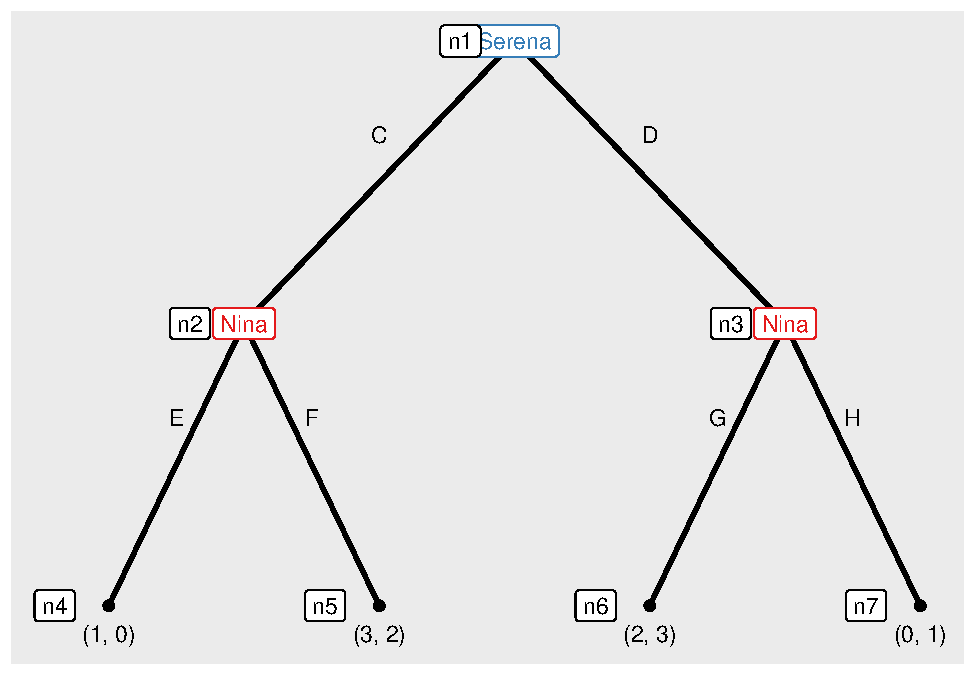
\includegraphics{aula_10_files/figure-latex/unnamed-chunk-1-1.pdf}

\hypertarget{fazer-quarta-rodada}{%
\section{fazer quarta rodada}\label{fazer-quarta-rodada}}

\hypertarget{generalizar-para-n-rodadas.}{%
\section{generalizar para n
rodadas.}\label{generalizar-para-n-rodadas.}}

\hypertarget{perceber-que-uxe0-medida-que-n-aumenta-vai-convergindo-para-12.-12.-se-tivermos-infinitas-rodadas-esse-uxe9-o-en.}{%
\section{perceber que à medida que n aumenta, vai convergindo para 1/2.
1/2. Se tivermos infinitas rodadas, esse é o
EN.}\label{perceber-que-uxe0-medida-que-n-aumenta-vai-convergindo-para-12.-12.-se-tivermos-infinitas-rodadas-esse-uxe9-o-en.}}

\hypertarget{apresentar-a-estrutura-do-jogo.}{%
\section{Apresentar a estrutura do
jogo.}\label{apresentar-a-estrutura-do-jogo.}}

Nosso jogo consiste então de: Jogadores: \(N = {1,2}\) Estratrégias:
para a jogadora que propõe, uma proposta de divisão da torta (ou do 1
real) para 1 e 2 respectivamente, do tipo \((x, 1-x), x \in [0,1]\).
Para a jogadora que recebe, se aceita ou rejeita a proposta. Logo,
temos: Quando a jogadora \(i\) propõe\$, \(S_i = (x, 1-x), x \in [0,1]\)
e quando a jogadora \(i\) recebe a proposta,
\(S_i = {aceita, rejeita}\). Payoffs: \(U_1(s_1, s_2) = \delta^t x\) e
\(U_2(s1, s2) = \delta^t (1-x)\).

\hypertarget{agora-modelo-bj}{%
\section{Agora, modelo BJ}\label{agora-modelo-bj}}

Vejam que quem joga por último obtém a maior parte do benefício para si.

\hypertarget{referuxeancias}{%
\subsection{Referências}\label{referuxeancias}}

Baron, D. P., \& Ferejohn, J. A. (1989). Bargaining in legislatures.
American political science review, 83(4), 1181-1206.

Rubinstein, A. (1982). Perfect equilibrium in a bargaining model.
Econometrica: Journal of the Econometric Society, 97-109.

\end{document}
